\documentclass[11pt,a4paper]{article}
\usepackage[margin=24mm]{geometry}\usepackage[T1]{fontenc}\usepackage{lmodern,amsmath,amssymb,booktabs,tabularx,longtable,graphicx,float,hyperref}
\hypersetup{colorlinks=true,urlcolor=blue,hypertexnames=true}\graphicspath{{figures/}}\setlength{\parindent}{0pt}\setlength{\parskip}{5pt}
\title{Supplementary Material\\Observer-Based Hybrid Position Holding for an Electrohydraulic Agricultural Hitch}
\author{Chenyu Cui, Peng Wang and Yucheng Zhang}\date{}
\renewcommand{\thetable}{S\arabic{table}}
\renewcommand{\thefigure}{S\arabic{figure}}
\begin{document}\maketitle
\section*{S1. Historical model and corrected interpretation}
The historical pressure-difference surrogate and V2 are separate models. The old surrogate has a virtual command-to-pressure relaxation, a retained-loss multiplier and a virtual accumulator/recharge proxy. Its paired pressure outputs are reconstructed rather than separately conserved. The implemented pressure loss is $\mathcal L=\kappa[1+g_T\max(T-25,0)]\max(d,0)/A$. Dimensional consistency requires $[\kappa]=\mathrm{m^2\,s^{-1}}$ so that $[\mathcal L]=\mathrm{Pa\,s^{-1}}$. The old physical leakage-flow interpretation and m$^3$ s$^{-1}$ Pa$^{-1}$ label are withdrawn. Old file identifiers are retained only to reproduce historical computations. The corrected coefficient-proxy inversion and a rate-dependent bound appear in Section 3.5. They do not identify physical leakage in V2.

The archived raw 0.10 MPa pressure-noise group (seeds 2060--2079) has 500 mm maximum steady error in every path, with mean steady RMSE 486.56 mm. A small reported downward drop of 0.033 mm in that group is not successful holding: the actuator travels to the upper stroke boundary. This illustrates why displacement drop alone is an insufficient acceptance metric. The V2 replay at the same absolute pressure-noise SD has 20/20 passes and no stroke hit, but its observer, reference and draw sequence also differ. This is a comparison of implementations, not a controlled attribution to chamber architecture alone.

\section*{S2. Measurement interface and original selection budget}
The full observer update, pressure command, saturation, integrators, switching order, hysteresis and timers are in Sections 3.2--3.3. Position correction is 0.08, velocity correction is $0.0005/h_c$, pressure filtering is 0.18 and effective-load smoothing is 0.005 per controller sample. Initial position and pressures equal the initial plant values, velocity is zero, and load starts at 9000 N. This initialization is a virtual-study assumption; it is not evidence of physical observer convergence. The effective load is clipped to [3000,20000] N in the controller. Nominal model coefficients remain fixed when true mechanical parameters are varied.

The 27 development candidates cross dwell $\{4,8,12\}$ s, support-error threshold $\{2.5,4,6\}$ mm and support-pressure threshold $\{0.18,0.30,0.45\}$ MPa, evaluated for 300 s on seeds 4100--4104. All pass five development paths. Ranking is lexicographic: maximum pass count, then minimum mean oil volume, mean mode changes and mean drop. Equal ties preserve enumeration order. No revision result changes the selected settings. The complete development table follows; quantities are virtual inputs or outputs, not hardware calibration.
Table~\ref{supp:longtable:1} provides the detailed supporting records.
\begin{longtable}{rrrrrr}\caption{Original development grid; every row passes 5/5.}\label{supp:longtable:1}\\\toprule Dwell (s)&Error (mm)&Deficit (MPa)&Oil (mL)&Switches&Drop (mm)\\\midrule\endfirsthead
\toprule Dwell (s)&Error (mm)&Deficit (MPa)&Oil (mL)&Switches&Drop (mm)\\\midrule\endhead
4 & 2.5 & 0.18 & 21.27 & 5.0 & 0.996 \\
4 & 2.5 & 0.30 & 15.50 & 3.4 & 1.222 \\
4 & 2.5 & 0.45 & 15.50 & 3.4 & 1.222 \\
4 & 4.0 & 0.18 & 21.27 & 5.0 & 0.996 \\
4 & 4.0 & 0.30 & 0.00 & 3.0 & 1.773 \\
4 & 4.0 & 0.45 & 0.00 & 3.0 & 1.773 \\
4 & 6.0 & 0.18 & 21.27 & 5.0 & 0.996 \\
4 & 6.0 & 0.30 & 0.00 & 3.0 & 1.773 \\
4 & 6.0 & 0.45 & 0.00 & 3.0 & 1.773 \\
8 & 2.5 & 0.18 & 25.44 & 5.0 & 0.845 \\
8 & 2.5 & 0.30 & 17.98 & 3.0 & 1.230 \\
8 & 2.5 & 0.45 & 17.98 & 3.0 & 1.230 \\
8 & 4.0 & 0.18 & 25.44 & 5.0 & 0.845 \\
8 & 4.0 & 0.30 & 0.00 & 3.0 & 1.754 \\
8 & 4.0 & 0.45 & 0.00 & 3.0 & 1.754 \\
8 & 6.0 & 0.18 & 25.44 & 5.0 & 0.845 \\
8 & 6.0 & 0.30 & 0.00 & 3.0 & 1.754 \\
8 & 6.0 & 0.45 & 0.00 & 3.0 & 1.754 \\
12 & 2.5 & 0.18 & 30.46 & 4.6 & 0.861 \\
12 & 2.5 & 0.30 & 20.82 & 3.0 & 1.188 \\
12 & 2.5 & 0.45 & 20.82 & 3.0 & 1.188 \\
12 & 4.0 & 0.18 & 30.46 & 4.6 & 0.861 \\
12 & 4.0 & 0.30 & 0.00 & 3.0 & 1.803 \\
12 & 4.0 & 0.45 & 0.00 & 3.0 & 1.803 \\
12 & 6.0 & 0.18 & 30.46 & 4.6 & 0.861 \\
12 & 6.0 & 0.30 & 0.00 & 3.0 & 1.803 \\
12 & 6.0 & 0.45 & 0.00 & 3.0 & 1.803 \\
\bottomrule\end{longtable}
\section*{S3. Original frozen statistics and uncertainty}
The submitted 20 paths use seeds 4120--4139, disjoint from development. Mean confidence intervals use $\bar z\pm t_{0.975,n-1}s/\sqrt n$, where $s$ is sample SD. These are intervals for seeded model-noise means, not hardware population intervals or pass-probability guarantees. No seed is removed for failure. Drop statistics require hold entry; every submitted path enters holding. The post-transition maximum error and pass screens include failed paths.
Table~\ref{supp:longtable:2} provides the detailed supporting records.
\begin{longtable}{p{.23\linewidth}p{.26\linewidth}rrr}\caption{Original frozen statistics and confidence intervals, including failed paths.}\label{supp:longtable:2}\\\toprule Chain & Metric & Mean & SD & 95\% CI\\\midrule\endfirsthead
\toprule Chain & Metric & Mean & SD & 95\% CI\\\midrule\endhead
PID--lock & Drop (mm) & 16.041 & 0.065 & 16.010--16.071 \\
PID--lock & RMSE (mm) & 8.232 & 0.115 & 8.178--8.286 \\
PID--lock & Max. error (mm) & 15.138 & 0.132 & 15.076--15.200 \\
PID--lock & Mode changes & 1.000 & 0.000 & 1.000--1.000 \\
PID--lock & Oil (mL) & 0.000 & 0.000 & 0.000--0.000 \\
SMC--lock & Drop (mm) & 15.995 & 0.055 & 15.969--16.021 \\
SMC--lock & RMSE (mm) & 9.174 & 0.175 & 9.092--9.256 \\
SMC--lock & Max. error (mm) & 16.227 & 0.199 & 16.134--16.320 \\
SMC--lock & Mode changes & 1.000 & 0.000 & 1.000--1.000 \\
SMC--lock & Oil (mL) & 0.000 & 0.000 & 0.000--0.000 \\
PID--accumulator & Drop (mm) & 3.441 & 0.249 & 3.325--3.558 \\
PID--accumulator & RMSE (mm) & 0.246 & 0.004 & 0.244--0.247 \\
PID--accumulator & Max. error (mm) & 6.960 & 0.219 & 6.858--7.063 \\
PID--accumulator & Mode changes & 26.800 & 5.872 & 24.052--29.548 \\
PID--accumulator & Oil (mL) & 25.538 & 1.200 & 24.977--26.100 \\
Observer hybrid & Drop (mm) & 1.849 & 0.156 & 1.776--1.922 \\
Observer hybrid & RMSE (mm) & 1.222 & 0.026 & 1.210--1.234 \\
Observer hybrid & Max. error (mm) & 8.435 & 0.219 & 8.332--8.537 \\
Observer hybrid & Mode changes & 13.100 & 0.447 & 12.891--13.309 \\
Observer hybrid & Oil (mL) & 1.019 & 4.559 & -1.114--3.153 \\
\bottomrule\end{longtable}
\section*{S4. Integration refinement and local boundedness checks}
Sensing, observer updates and commanded inputs remain on the 10 ms grid. Only the plant is substepped at 10, 5, 2.5 or 1 ms; the measurement draws are identical on common controller samples. Pressure updates use the old position/velocity and the updated spool, then the mechanical update uses the new pressures, and position uses the new velocity. This sequential explicit scheme and its pressure/stroke projections are retained. It is not an adaptive error-controlled solver. Pressure discrepancies below aggregate both chambers on all 10 ms sample endpoints against the 1 ms run. Maxima may include a switching-time displacement and are not an estimate of local truncation order.
Table~\ref{supp:table:1} provides the detailed supporting records.
\begin{table}[H]\centering\caption{Full-horizon 10 ms versus 1 ms pressure and drop differences.}\label{supp:table:1}\begin{tabular}{rrrr}\toprule Seed&Pressure RMS (MPa)&Max. difference (MPa)&Drop difference (mm)\\\midrule
4300 & 0.0638 & 0.1510 & 0.1990 \\
4301 & 0.0642 & 0.1657 & 0.1120 \\
4302 & 0.0640 & 0.1583 & 0.2394 \\
4303 & 0.0633 & 0.1543 & -0.0326 \\
4304 & 0.0633 & 0.1522 & 0.2357 \\
\bottomrule\end{tabular}\end{table}
The event-clipped RK4 audit keeps controller, observer and measurement updates on the 10 ms grid and changes only the virtual-plant update. Five predeclared seeds were run at 1.0 and 0.5 ms; all paths passed. The mean hold drops were 1.628 and 1.585 mm, and the mean worst post-transition errors were 8.503 and 8.502 mm. The mean absolute per-seed difference in worst error was 0.0023 mm and the mean absolute hold-drop difference was 0.046 mm. These results support fine-step numerical convergence of the refined arm, while switching and friction remain sources of hold-drop sensitivity.
The corresponding numerical summary is reported in Table 6 of the main article; it is not duplicated here.
The projected-model velocity bound is independent of mode but depends on imposed pressure/stroke limits. It is deliberately too loose for a 10 mm guarantee. For the unprojected local calculation at $\bar x=0.35$ m, nominal $C_l=5\times10^{-14}$ m$^3$ s$^{-1}$ Pa$^{-1}$ and 25 $^\circ$C, the frozen-volume matrix in Section 3.4 has eigenvalues approximately $-6.23\times10^{-6}$ and $-0.918\pm73.08i$ s$^{-1}$. The slow pole exposes weak leakage-driven restoration rather than precise locking. The Lyapunov argument is in fixed consistent coordinates, not a physical-energy interpretation of a mixed-unit Euclidean norm. The result concerns bounded forcing and fixed volumes, with no claim that the nonlinear trajectory remains in its local neighborhood.

\section*{S5. Noise activation, storage and historical alignment}
Independent Gaussian pressure noise is added before the V2 internal pressure filter; no new external low-pass filter is inserted. Position noise stays at 1.5 mm SD in the pressure-only sweep. The separate joint-noise case doubles both SDs. Dwell limits mode changes but does not prevent persistent positive support commands during a latched support mode. Pressure/position fluctuations change pressure balance and gate crossings, explaining the large change in oil volume from a near-zero nominal denominator. Gas pressure, cumulative discharge, active time and mode occupancy are recorded; energy consumption and valve wear are not inferred from these proxies.
Table~\ref{supp:table:2} provides the detailed supporting records.
\begin{table}[H]\centering\caption{Five-path noise-group activity and storage extrema.}\label{supp:table:2}\begin{tabularx}{\linewidth}{Xrrrr}\toprule Noise input & Pass & Active time (s) & Mean oil (mL) & Min. gas (MPa)\\\midrule
Nominal & 5/5 & 0.00 & 0.00 & 14.000 \\
Both SDs doubled & 5/5 & 6.23 & 39.92 & 13.553 \\
Pressure SD 0.10 MPa & 5/5 & 18.51 & 98.76 & 13.325 \\
Pressure SD 0.20 MPa & 5/5 & 177.44 & 298.04 & 12.204 \\
Pressure SD 0.50 MPa & 5/5 & 450.62 & 447.11 & 11.497 \\
Pressure SD 1.00 MPa & 2/5 & 479.06 & 454.13 & 11.466 \\
\bottomrule\end{tabularx}\end{table}
The ten original jointly doubled-noise paths were replayed with diagnostic logging before the timestamp-schema correction; all original fields match exactly in that frozen replay. Mean support-command active time is 10.391 s (SD 5.196 s), mean oil volume 61.982 mL (SD 28.408 mL), and the minimum gas pressure across the group is 13.337 MPa. Every path passes the original screen and has no stroke hit. Figure 10 of the main article shows the first original stress seed 4160, against a same-seed nominal replay, so that the original discharge increase has a direct trajectory diagnosis rather than being explained only through a new seed set.


The aligned 20-path historical-noise replay gives mean drop 1.860 mm (95\% interval 1.774--1.946), worst error 8.723 mm, and mean oil 105.36 mL. Its larger discharge is compatible with passing the position screen. Seeds and SD match the old experiment, but the stochastic samples, plant, reference and internal observer do not. An architecture-only noise-robustness causal claim is therefore withheld.
\section*{S6. Parameter provenance and revision overrides}
The original 45-row parameter manifest is supplied without rewriting historical coverage labels. Every number is a researcher-defined theoretical input. The new ledger records additional true-plant overrides, integration substeps, observer-removal arms and noise scales separately. Hydraulic area, dead volume, effective bulk modulus, flow area and dead zone have not been independently identified. A declared range in the submitted table did not by itself document a performed test. The new mechanical runs vary one true coefficient at a time and keep controller/observer inputs nominal; they cannot establish robustness over all simultaneous combinations.

\section*{S7. Reproduction and integrity}
The public repository contains the current model source, declared parameters, clean manuscript source and a minimal source-only runner. It deliberately excludes frozen JSON evidence, historical audit ledgers, checkpoints, reviewer correspondence and submission archives. The runner creates a new external workspace and writes newly generated JSON there; it does not read any historical result file. The values in this supplementary PDF remain the published numerical record, while a fresh run is a source-level theoretical recomputation rather than a byte-for-byte replay of an omitted archive.
\begin{verbatim}
./reproduce_paper1.sh --workspace /tmp/paper1-reproduction
\end{verbatim}
The short runner evaluates one seeded hybrid and PID virtual trajectory for an externally selected duration. It is intended to verify that the public source imports and executes from a clean checkout; it is not a replacement for the finite numerical evidence reported in the published article and does not claim hardware validation.
\section*{S8. Paired RK4 comparators and joint mechanical vertices}
The strengthening protocol fixes all 70 rows before computation: 30 nominal comparator rows and 40 joint-vertex rows. Ten nominal hybrid rows are reused from the earlier RK4 audit, so 60 new trajectories are computed. Each path lasts 1800 s, with controller/observer/noise updates at 10 ms. The two PID arms use exactly the same five seeds and plant integrator as the hybrid; the matched arm changes only the declared latch and discharge-gating semantics. The joint screen crosses all eight $\{0.7,1.3\}^3$ mass/damping/stiffness vertices with five seeds, a 1 ms RK4 plant step and fixed nominal control coefficients. The published tables report the resulting summaries; raw checkpoints and generated path files are not part of the public source snapshot. These vertices do not certify the full box or an uncertainty probability distribution. Endpoint projections do not locate event roots or establish a fourth-order rate for this nonsmooth system.
The corresponding numerical summary is reported in Table 7 of the main article; it is not duplicated here.

The corresponding numerical summary is reported in Table 9 of the main article; it is not duplicated here.
Table~\ref{supp:table:3} provides the detailed supporting records.
\begin{table}[H]\centering\small
\caption{Paired PID-minus-hybrid differences in hold drop and RMSE with Student-$t$ 95\% intervals, five paired seeds per row. Intervals concern seeded noise at the declared plant, not uncertainty in model structure or hardware performance.}\label{supp:table:3}
\begin{tabularx}{\linewidth}{@{}>{\raggedright\arraybackslash}p{.29\linewidth}*{3}{>{\centering\arraybackslash}X}@{}}\toprule
PID arm & Step (ms) & Drop difference (mm), 95\% CI & RMSE difference (mm), 95\% CI\\\midrule
Original PID & 1.0 & 1.374 [1.149, 1.599] & -0.929 [-0.962, -0.896] \\
Matched PID & 1.0 & 1.400 [1.147, 1.652] & -0.929 [-0.962, -0.896] \\
Original PID & 0.5 & 1.358 [1.091, 1.625] & -0.941 [-0.966, -0.917] \\
Matched PID & 0.5 & 1.368 [1.106, 1.630] & -0.941 [-0.965, -0.917] \\
\bottomrule\end{tabularx}\end{table}
\begin{verbatim}
% Historical audit command omitted from the public source snapshot.
% Historical audit command omitted from the public source snapshot.
\end{verbatim}
\section*{S9. Physical-system and combined-stress audit}
Figure 1 of the main article records the physical-system abstraction used by the V2 equations. The piston coordinate is the simulated displacement; an implement displacement would require an external linkage map and is not calibrated here. The observer uses noisy position and chamber-pressure measurements at 10 ms. The symmetric equal-area assumption is retained as a declared virtual-model boundary.
The corresponding graphic is Figure 1 of the main article and is not duplicated here.

The combined stress protocol was declared before execution and uses load changes at 0, 60, 300, 600, 900 and 1200 s, five seeds (4400--4404), the 1800 s reference and the unchanged 10 ms observer/controller. The nominal arm uses the declared leakage coefficient. The second arm multiplies it by five; the third uses the same fivefold coefficient with the accumulator valve disabled. Each arm contains five traces and no case is selected after observing its result.
The corresponding numerical summary is reported in Table 2 of the main article; it is not duplicated here.
The enabled fivefold arm reached a minimum accumulator pressure of 13.59 MPa and used 36.02 mL mean oil on these traces; the nominal arm used 38.13 mL. The disabled arm also passed 5/5, so this protocol does not show that the accumulator is necessary. It does show the requested ablation result and makes the limitation explicit: stronger storage-demanding disturbances, recharge dynamics and calibrated leakage remain untested.
The corresponding graphic is Figure 5 of the main article and is not duplicated here.
The friction-mismatch extension uses the same five seeds, repeated-load schedule and fivefold virtual leakage. In the 0.7$\times$ arm the true-plant viscous, Coulomb and Stribeck terms are all reduced together; in the 1.3$\times$ arm they are all increased together. The observer and controller retain nominal force-balance coefficients; neither explicitly compensates Coulomb/Stribeck friction, whose effects can enter the effective-load estimate. Both arms enter and pass on 5/5 paths, with worst errors of 8.63 and 8.65 mm and worst drops of 2.88 and 2.99 mm, respectively. S10 adds independent friction amplitudes/velocity scales and interacting parameters. Neither finite screen identifies a physical friction law or guarantees the full region.
The corresponding numerical summary is reported in Table 10 of the main article; it is not duplicated here.
\section*{S10. Independent tuning and uncertainty audits}

\paragraph{Additional independent risk-closure protocol.}
The frozen submitted gains remain distinct from a new equal-budget development comparison. Each policy receives nine candidates. Tracking multipliers are $g_t\in\{0.7,1,1.3\}$; accumulator multipliers are $g_a\in\{0.5,1,1.5\}$. The multiplier $g_t$ scales the 650 and 90 feedback gains and the PID integral gain 20, but leaves reference feedforward unchanged; $g_a$ scales the complete accumulator command before saturation. Both policies use the same $\pm0.10$ main-valve authority, 8 s dwell and mode-gated discharge. Mode-request thresholds remain policy-specific. Thus authority, timing and search effort are matched without making the policies identical. Three development seeds (4600--4602), 300 s paths and 1 ms RK4 are used per candidate. The development load schedule is $(0,9),(60,14),(100,10),(160,16),(220,11),(260,15)$ kN with fivefold leakage. Candidates are ranked by failure count, then mean $J=\Delta_h/10+\mathrm{RMSE}/10+V_{acc}/500+N_{sw}/225$, using mm and mL. These fixed engineering normalizations express one preference, not universal utility weights. All candidates and their four-objective nondominated subset are retained. Selection is recorded before the independent 1800 s evaluation on seeds 4700--4709, using the full repeated-load schedule at both 1 and 0.5 ms. No validation outcome changes selection. Both policies share each seed's measurement sequence and initial plant state. This finite grid is not a global optimization or a comparison against all robust-control methods.

A separate convergence screen repeats nominal leakage, fivefold leakage, accumulator-disabled and linked $0.7/1.3\times$ friction arms at 1 and 0.5 ms on seeds 4400--4402, without retuning the submitted controller. A 24-path stratified interior screen uses new seeds 4800--4823 and independently permuted bins for 12 simultaneous inputs: mass, viscous damping, stiffness, Coulomb friction, Stribeck amplitude and velocity scale, bulk modulus, spool lag, leakage multiplier, accumulator flow coefficient, pressure-noise amplitude and position bias. The intervals and all sampled inputs are supplied in S10. These are virtual-design intervals, not calibrated distributions. The controller retains the original gains and nominal force-balance coefficients. It contains no explicit Coulomb/Stribeck compensation; these unmodeled terms can enter its effective-load estimate. Independent friction magnitudes and velocity scales test more than a linked scaling, but the functional friction law itself remains fixed.


The current metric schema records the confirmation sample and first post-update endpoint separately. Historical numerical outputs are unchanged; the old start label is retained as legacy metadata. A four-chain regression on seed 4120 reproduces every historical output field except the corrected start timestamp. The confirmation gate counts 100 samples; it is not reinterpreted as a continuous-time crossing. The new metric records the start position, minimum hold position and sample count so that the reported drop is directly checkable.

\paragraph{Scope of mathematical statements.} The sequential projected-state recurrence uses the actual friction bound and integration step of each plant. It bounds numerical states without guaranteeing millimeter accuracy. Positive parameters satisfy the frozen-volume Routh test pointwise, but the corresponding Lyapunov matrix depends on those parameters. Neither argument proves stability of the nonlinear switched unprojected plant. The RK4 and uncertainty results are simulation evidence, not replacements for such a proof.

\paragraph{Declared simultaneous intervals.} Mass 840--1560 kg; viscous coefficient 1540--2860 N s m$^{-1}$; stiffness 12600--23400 N m$^{-1}$; Coulomb friction 595--1105 N; Stribeck amplitude 245--455 N; Stribeck velocity 0.0028--0.0052 m s$^{-1}$; bulk modulus 0.14--0.26 GPa; spool lag 35--65 ms; leakage multiplier 1--10; accumulator-flow multiplier 0.5--1.5; pressure-noise multiplier 1--4; position bias $-2$ to $+2$ mm. Seed 48191 fixes stratification and independent bin permutations. The 24 input vectors are summarized in the published tables. The original submitted hybrid is used; these data do not tune a new robust controller.

Table~\ref{supp:table:4} provides the detailed supporting records.
\begin{table}[H]\centering\small
\caption{Complete development grid. Each candidate has three 300 s development paths. The nondominated flag uses drop, RMSE, oil and switching jointly.}\label{supp:table:4}
\begin{tabularx}{\linewidth}{@{}>{\raggedright\arraybackslash}p{.13\linewidth}*{7}{>{\centering\arraybackslash}X}@{}}\toprule
Policy & ID & $g_t/g_a$ & Fail & Mean $J$ & Drop & RMSE & Nondom.\\\midrule
Hybrid & 0 & 0.7/0.5 & 3 & 0.4695 & 2.478 & 1.411 & No\\
Hybrid & 1 & 0.7/1.0 & 3 & 0.5016 & 2.493 & 1.420 & No\\
Hybrid & 2 & 0.7/1.5 & 3 & 0.5234 & 2.479 & 1.411 & No\\
Hybrid & 3 & 1.0/0.5 & 0 & 0.4295 & 2.254 & 1.200 & Yes\\
Hybrid & 4 & 1.0/1.0 & 0 & 0.4577 & 2.276 & 1.204 & No\\
Hybrid & 5 & 1.0/1.5 & 0 & 0.4823 & 2.307 & 1.211 & No\\
Hybrid & 6 & 1.3/0.5 & 0 & 0.4521 & 2.471 & 1.127 & Yes\\
Hybrid & 7 & 1.3/1.0 & 0 & 0.4880 & 2.489 & 1.108 & Yes\\
Hybrid & 8 & 1.3/1.5 & 0 & 0.5209 & 2.514 & 1.165 & No\\
PID & 0 & 0.7/0.5 & 2 & 0.7174 & 3.990 & 1.174 & No\\
PID & 1 & 0.7/1.0 & 2 & 0.7998 & 3.870 & 1.151 & No\\
PID & 2 & 0.7/1.5 & 2 & 0.8504 & 3.799 & 1.136 & No\\
PID & 3 & 1.0/0.5 & 0 & 0.6106 & 3.843 & 0.891 & No\\
PID & 4 & 1.0/1.0 & 0 & 0.6713 & 3.748 & 0.874 & No\\
PID & 5 & 1.0/1.5 & 0 & 0.7160 & 3.678 & 0.864 & No\\
PID & 6 & 1.3/0.5 & 0 & 0.5476 & 3.666 & 0.748 & Yes\\
PID & 7 & 1.3/1.0 & 0 & 0.5968 & 3.606 & 0.738 & Yes\\
PID & 8 & 1.3/1.5 & 0 & 0.6346 & 3.560 & 0.729 & Yes\\
\bottomrule\end{tabularx}\end{table}

Table~\ref{supp:table:5} provides the detailed supporting records.
\begin{table}[H]\centering\small
\caption{Paired matched-PID minus hybrid differences, independent ten-seed test. Student-t intervals summarize seeded model noise; they do not represent parameter or physical uncertainty.}\label{supp:table:5}
\begin{tabularx}{\linewidth}{@{}>{\raggedright\arraybackslash}p{.15\linewidth}*{3}{>{\centering\arraybackslash}X}@{}}\toprule
Step (ms) & Quantity & Mean difference & 95\% interval\\\midrule
1.0 & Drop (mm) & 1.4651 & [1.2326, 1.6976]\\
1.0 & RMSE (mm) & -0.9519 & [-0.9633, -0.9405]\\
1.0 & Oil (mL) & 10.7885 & [7.0132, 14.5638]\\
1.0 & Changes & -47.5000 & [-48.1079, -46.8921]\\
0.5 & Drop (mm) & 1.4470 & [1.2021, 1.6920]\\
0.5 & RMSE (mm) & -0.9594 & [-0.9719, -0.9469]\\
0.5 & Oil (mL) & 11.4952 & [6.5113, 16.4791]\\
0.5 & Changes & -47.2000 & [-47.8574, -46.5426]\\
\bottomrule\end{tabularx}\end{table}

Table~\ref{supp:table:6} provides the detailed supporting records.
\begin{table}[H]\centering\small
\caption{Every joint interior sample, submitted hybrid at 1 ms RK4. Full input vectors accompany each checkpoint.}\label{supp:table:6}
\begin{tabularx}{\linewidth}{@{}>{\raggedright\arraybackslash}p{.12\linewidth}*{6}{>{\centering\arraybackslash}X}@{}}\toprule
Seed & Entry & Drop (mm) & Max error (mm) & Relief & Stroke & Screen\\\midrule
4800 & Yes & 2.640 & 9.928 & 0 & 0 & Pass\\
4801 & Yes & 2.684 & 6.628 & 0 & 0 & Pass\\
4802 & Yes & 3.265 & 9.232 & 0 & 0 & Pass\\
4803 & Yes & 2.470 & 8.661 & 0 & 0 & Pass\\
4804 & Yes & 2.389 & 6.468 & 0 & 0 & Pass\\
4805 & Yes & 1.899 & 8.465 & 0 & 0 & Pass\\
4806 & Yes & 2.379 & 10.155 & 0 & 0 & Fail\\
4807 & Yes & 2.054 & 6.932 & 0 & 0 & Pass\\
4808 & Yes & 1.585 & 9.288 & 0 & 0 & Pass\\
4809 & Yes & 2.396 & 7.314 & 0 & 0 & Pass\\
4810 & Yes & 2.819 & 9.279 & 0 & 0 & Pass\\
4811 & Yes & 2.224 & 8.047 & 0 & 0 & Pass\\
4812 & Yes & 2.179 & 8.056 & 0 & 0 & Pass\\
4813 & Yes & 2.058 & 7.372 & 0 & 0 & Pass\\
4814 & Yes & 3.659 & 7.839 & 0 & 0 & Pass\\
4815 & Yes & 2.208 & 6.563 & 0 & 0 & Pass\\
4816 & Yes & 1.748 & 9.395 & 0 & 0 & Pass\\
4817 & Yes & 2.423 & 5.735 & 0 & 0 & Pass\\
4818 & Yes & 2.479 & 9.330 & 0 & 0 & Pass\\
4819 & Yes & 2.966 & 9.587 & 0 & 0 & Pass\\
4820 & Yes & 1.244 & 5.993 & 0 & 0 & Pass\\
4821 & Yes & 2.056 & 10.004 & 0 & 0 & Fail\\
4822 & Yes & 2.598 & 9.724 & 0 & 0 & Pass\\
4823 & Yes & 2.734 & 7.555 & 0 & 0 & Pass\\
\bottomrule\end{tabularx}\end{table}

\begin{verbatim}
% Historical audit command omitted from the public source snapshot.
% Historical audit command omitted from the public source snapshot.
\end{verbatim}

\section*{S11. Verified active comparison and new joint design}

\paragraph{Active nonlinear comparison and verified execution.}
The active sliding-mode (SMC) chain uses $1200\tanh[(18e+e_v)/0.006]$ N with the common observer, pressure PI, nominal force-balance coefficients and $\pm0.10$ holding authority, without the PID position integral. The main valve remains active during holding. The support threshold is $e>2$ mm. Its accumulator command is
\[
u_{acc}=\operatorname{clip}_{[0,1]}[80g_a\max(e-0.001,0)].
\]
Discharge additionally requires the latched ACCUMULATOR label. Both active baselines explicitly receive the same 8 s latch argument; their initial FINE\_TRIM label is retained until the latch expires. The hybrid has its stated policy-specific hysteresis and the same 8 s minimum dwell. The control interfaces and budgets are matched, while the decision rules remain different. This is an executable boundary-layer comparator informed by the sliding-mode family (see the main-article sliding-mode references); it does not reproduce a published adaptive design or prove reaching of the full saturated loop.

A final execution audit found that an earlier SMC runner supplied zero rather than 8 s to the latch argument, also bypassing mode-gated discharge. Its records remain archived as an unlatched diagnostic and are excluded from matched-baseline claims. A separately frozen correction repeats all nine SMC candidates on the same development seeds 4600--4602, 300 s schedule, 1 ms RK4 and unchanged scalar objective. Selection uses only those corrected development outcomes. Corrected SMC replays of common nominal seeds 4700--4709 at 1 and 0.5 ms, known vectors 4800--4823 and previously examined vectors 4900--4923 are follow-up checks, not fresh holdouts. Changes relative to the unlatched arm combine execution correction with reselection; they do not isolate a causal effect of dwell alone.

\paragraph{Separate accuracy preference and new joint verification.}
The scalar-selected hybrid and PID remain frozen at $(g_t,g_a)=(1,0.5)$ and $(1.3,0.5)$. The margin hybrid remains the original development-grid choice $(1.3,0.5)$: require no development failure and worst development error $\le8$ mm, then minimize the same $J$ and candidate ID. Its 2 mm reserve is a heuristic for the stated bias amplitude, not a total observer-error bound. No result from a joint design changes these choices. Corrected SMC selection applies the same nine-candidate rule, and its eligibility under the 8 mm constraint is reported separately. Development-only weight profiles remain sensitivity checks rather than test-based tuning.

Before corrected development, random seed 51191 freezes 24 new stratified vectors over the same twelve intervals, with noise seeds 5100--5123. All four policy instances face identical true-plant overrides, measurement-noise sequences, reference, repeated-load schedule, initial state and 1 ms RK4 integration. The measured values themselves differ with each policy's plant trajectory. These are the new joint verification outcomes; the earlier 4900-series outcomes are identified as previous-design follow-up. The new correction contains 27 development paths and 164 full-horizon paths: 68 corrected SMC follow-ups and 96 new four-policy joint paths. The published tables summarize the selection and failed paths. The intervals are numerical design choices without physical-frequency interpretation; generated checkpoints are not part of the public source snapshot.


\paragraph{Evidence versions.} The earlier 255-path extension remains a historical analysis record. That runner passed the 8 s argument only to PID; its active-SMC paths had zero baseline dwell and ungated discharge. Earlier claims that those SMC paths matched the latch/gate are withdrawn. The corrected dispatcher recorded the actual arguments in the private audit. The hydraulic/controller source is unchanged; the correction is in experiment dispatch. A configuration flag named matched is not itself evidence that the function received the requested arguments.

Table~\ref{supp:table:7} provides the detailed supporting records.
\begin{table}[H]\centering\small
\caption{Roles of corrected paths. Development precedes selection; the new joint vectors are frozen before corrected development. The original 158-path and earlier 255-path ledgers remain historical evidence.}\label{supp:table:7}
\begin{tabularx}{\linewidth}{@{}>{\raggedright\arraybackslash}p{.27\linewidth}*{4}{>{\centering\arraybackslash}X}@{}}\toprule
Family & Seeds & Duration (s) & Paths & Role\\\midrule
SMC development & 4600--4602 & 300 & 27 & Selection only\\
SMC common nominal & 4700--4709 & 1800 & 20 & Known-protocol follow-up; two steps\\
SMC known vectors & 4800--4823 & 1800 & 24 & Known-design follow-up\\
SMC previous joint & 4900--4923 & 1800 & 24 & Previous-design follow-up\\
Four-policy new joint & 5100--5123 & 1800 & 96 & New stratified verification\\
\bottomrule\end{tabularx}\end{table}

\paragraph{Position-filter bias and moment bounds.}
The implemented position/velocity filter has the exact stored-state recursion
\begin{equation}
 z_{k+1}=Fz_k+By_k,\qquad
 F=\begin{bmatrix}1-\alpha&h\\-\beta/h&1\end{bmatrix},\quad
 B=\begin{bmatrix}\alpha\\\beta/h\end{bmatrix},\quad
 (h,\alpha,\beta)=(0.01,0.08,0.0005),
\end{equation}
where $z=(\hat x,\hat v)^\top$ and $y$ is measured position. Its poles are 0.926834 and 0.993166. Bounded measurement inputs therefore give bounded filter states, but the DC response to a constant measured position is $(I-F)^{-1}B=(1,0)^\top$: constant position bias is retained. For the additive iid measurement-noise component with a frozen input trajectory, $P=FPF^\top+\sigma_x^2BB^\top$ gives position standard deviation $0.211675\sigma_x$ (0.318 mm at the nominal 1.5 mm raw SD). This is a filter-component calculation, not the covariance of the feedback-connected hydraulic loop. The identity $x_r-x=(x_r-\hat x)+(\hat x-x)$ shows why estimated error alone cannot certify true accuracy without an observer-error bound. The 2 mm design reserve accounts heuristically for one bias component; motion transients, pressure/load estimation and unbounded Gaussian samples prevent interpreting it as a guaranteed total error budget.

A limited moment bound is still available under the declared projections. Since true position is in $[0,L]$, bounded bias and finite measurement-noise variance give a uniformly finite $L_2$ norm of $y_k$. After expressing stored states and measurements in fixed dimensionless units, Schur stability supplies $C<\infty$ and $0<r<1$ such that $\|F^j\|\le Cr^j$. Minkowski's inequality then yields
\begin{equation}
 \|z_k\|_{L_2}\le Cr^k\|z_0\|_{L_2}
 +\frac{C\|B\|}{1-r}\sup_i\|y_i\|_{L_2}.
\end{equation}
This proves bounded second moments of this filter under projected-position inputs, including finite-variance Gaussian noise; it does not require feedback-input independence. The pressure filters have pole 0.82, and effective-load smoothing has pole 0.995 with input formed from those filters and a finite difference of $\hat v$, so their second moments are also bounded under bounded projected pressures and finite pressure-noise variance. Clipped control outputs and integrators remain bounded separately. These moment bounds establish neither a deterministic sample-path accuracy bound nor asymptotic tracking, invariance of the unprojected plant, or nonlinear switched stability.



Table~\ref{supp:table:8} provides the detailed supporting records.
\begin{table}[H]\centering\small
\caption{Corrected active-SMC development, nine candidates and three paths per candidate. Failures are ranked first, then mean J and candidate ID. Oil is mL; drop and RMSE are mm.}\label{supp:table:8}
\begin{tabularx}{\linewidth}{@{}>{\raggedright\arraybackslash}p{.08\linewidth}*{7}{>{\centering\arraybackslash}X}@{}}\toprule
ID & $g_t/g_a$ & Fail & Mean $J$ & Drop & RMSE & Oil & Changes\\\midrule
0 & 0.7/0.5 & 0 & 0.4401 & 2.678 & 0.684 & 36.398 & 7.000\\
1 & 0.7/1.0 & 0 & 0.4780 & 2.564 & 0.670 & 61.757 & 7.000\\
2 & 0.7/1.5 & 0 & 0.5105 & 2.509 & 0.659 & 81.302 & 7.000\\
3 & 1.0/0.5 & 0 & 0.3648 & 2.325 & 0.545 & 23.324 & 7.000\\
4 & 1.0/1.0 & 0 & 0.3938 & 2.260 & 0.537 & 41.515 & 7.000\\
5 & 1.0/1.5 & 0 & 0.4096 & 2.213 & 0.532 & 53.419 & 6.333\\
6 & 1.3/0.5 & 0 & 0.3038 & 1.991 & 0.479 & 14.309 & 6.333\\
7 & 1.3/1.0 & 0 & 0.3242 & 1.954 & 0.476 & 26.523 & 6.333\\
8 & 1.3/1.5 & 0 & 0.3451 & 1.951 & 0.473 & 37.256 & 6.333\\
\bottomrule\end{tabularx}\end{table}

Across 81 development-only weight profiles, corrected SMC candidate frequencies are 6: 81. These are descriptive counts, not probabilities. Under the 8 mm development reserve its selected candidate is 6. The original hybrid/PID weight profiles remain in the earlier ledger and do not change their gains.

Table~\ref{supp:table:9} provides the detailed supporting records.
\begin{table}[H]\centering\small
\caption{Corrected SMC paired nominal steps; measurement/control updates remain at 10 ms. Means are shown except worst error.}\label{supp:table:9}
\begin{tabularx}{\linewidth}{@{}>{\raggedright\arraybackslash}p{.12\linewidth}*{6}{>{\centering\arraybackslash}X}@{}}\toprule
Step (ms) & Pass & Drop (mm) & RMSE (mm) & Oil (mL) & Changes & Worst error (mm)\\\midrule
1.0 & 10/10 & 2.037 & 0.252 & 13.856 & 5.800 & 5.866\\
0.5 & 10/10 & 1.992 & 0.251 & 13.620 & 5.600 & 5.858\\
\bottomrule\end{tabularx}\end{table}

The archived unlatched nominal SMC at 0.5 ms had means 1.901 mm drop, 0.248 mm RMSE, 45.54 mL discharge and 36.6 changes. Those values concern its old (1.3,1.5) selection. The corrected candidate is (1.3,0.5); execution correction and reselection are not a one-factor causal comparison.

Table~\ref{supp:table:10} provides the detailed supporting records.
\begin{table}[H]\centering\small
\caption{Paired other-policy minus corrected-SMC differences on common nominal noise seeds. Positive values favor corrected SMC for that objective. Student-t intervals are descriptive model-design summaries, without physical-population or simultaneous-inference meaning.}\label{supp:table:10}
\begin{tabularx}{\linewidth}{@{}>{\raggedright\arraybackslash}p{.23\linewidth}*{3}{>{\centering\arraybackslash}X}@{}}\toprule
Other policy & Quantity & Mean difference & Descriptive 95\% interval\\\midrule
Scalar hybrid & Drop (mm) & 0.116 & [-0.213, 0.446]\\
Scalar hybrid & RMSE (mm) & 1.022 & [1.009, 1.035]\\
Scalar hybrid & Oil (mL) & 10.171 & [5.038, 15.303]\\
Scalar hybrid & Changes & 48.600 & [47.577, 49.623]\\
Active PID & Drop (mm) & 1.563 & [1.335, 1.791]\\
Active PID & RMSE (mm) & 0.062 & [0.059, 0.066]\\
Active PID & Oil (mL) & 21.666 & [19.272, 24.059]\\
Active PID & Changes & 1.400 & [0.709, 2.091]\\
Margin hybrid & Drop (mm) & 0.033 & [-0.274, 0.341]\\
Margin hybrid & RMSE (mm) & 0.953 & [0.933, 0.973]\\
Margin hybrid & Oil (mL) & 139.534 & [128.721, 150.347]\\
Margin hybrid & Changes & 48.400 & [46.641, 50.159]\\
\bottomrule\end{tabularx}\end{table}

Table~\ref{supp:table:11} provides the detailed supporting records.
\begin{table}[H]\centering\small
\caption{Paired other-policy minus corrected-SMC differences on new stratified joint design. Positive values favor corrected SMC for that objective. Student-t intervals are descriptive model-design summaries, without physical-population or simultaneous-inference meaning.}\label{supp:table:11}
\begin{tabularx}{\linewidth}{@{}>{\raggedright\arraybackslash}p{.23\linewidth}*{3}{>{\centering\arraybackslash}X}@{}}\toprule
Other policy & Quantity & Mean difference & Descriptive 95\% interval\\\midrule
Scalar hybrid & Drop (mm) & 0.377 & [0.069, 0.686]\\
Scalar hybrid & RMSE (mm) & 0.325 & [0.097, 0.554]\\
Scalar hybrid & Oil (mL) & 161.305 & [116.449, 206.161]\\
Scalar hybrid & Changes & 67.792 & [54.756, 80.827]\\
Active PID & Drop (mm) & 1.828 & [1.697, 1.959]\\
Active PID & RMSE (mm) & 0.021 & [0.007, 0.034]\\
Active PID & Oil (mL) & 20.324 & [17.849, 22.799]\\
Active PID & Changes & 1.250 & [0.832, 1.668]\\
Margin hybrid & Drop (mm) & 0.093 & [-0.127, 0.313]\\
Margin hybrid & RMSE (mm) & 0.220 & [0.025, 0.416]\\
Margin hybrid & Oil (mL) & 231.548 & [207.015, 256.081]\\
Margin hybrid & Changes & 82.417 & [67.240, 97.594]\\
\bottomrule\end{tabularx}\end{table}

Table~\ref{supp:table:12} provides the detailed supporting records.
\begin{table}[H]\centering\small
\caption{Every new joint maximum error in mm. Screen order is scalar hybrid / PID / corrected SMC / margin hybrid; P requires all declared criteria. The published tables retain the summarized vectors and metrics.}\label{supp:table:12}
\begin{tabularx}{\linewidth}{@{}>{\raggedright\arraybackslash}p{.09\linewidth}*{5}{>{\centering\arraybackslash}X}@{}}\toprule
Seed & Scalar hybrid & Active PID & Active SMC & Margin hybrid & Screens\\\midrule
5100 & 9.068 & 6.211 & 6.530 & 7.684 & P/P/P/P\\
5101 & 8.467 & 5.498 & 5.810 & 6.977 & P/P/P/P\\
5102 & 8.670 & 5.765 & 6.081 & 7.242 & P/P/P/P\\
5103 & 9.277 & 6.181 & 6.498 & 7.658 & P/P/P/P\\
5104 & 9.463 & 6.490 & 6.865 & 7.957 & P/P/P/P\\
5105 & 7.565 & 4.589 & 4.911 & 6.067 & P/P/P/P\\
5106 & 8.075 & 5.169 & 5.488 & 6.647 & P/P/P/P\\
5107 & 9.850 & 7.068 & 7.377 & 8.544 & P/P/P/P\\
5108 & 9.754 & 6.881 & 7.203 & 8.355 & P/P/P/P\\
5109 & 9.972 & 7.059 & 7.310 & 8.540 & P/P/P/P\\
5110 & 9.872 & 6.830 & 7.155 & 8.310 & P/P/P/P\\
5111 & 9.353 & 6.209 & 6.512 & 7.679 & P/P/P/P\\
5112 & 6.337 & 4.155 & 3.734 & 4.887 & P/P/P/P\\
5113 & 7.371 & 4.445 & 4.746 & 5.923 & P/P/P/P\\
5114 & 7.562 & 4.556 & 4.875 & 6.023 & P/P/P/P\\
5115 & 7.405 & 4.453 & 4.762 & 5.919 & P/P/P/P\\
5116 & 7.184 & 4.272 & 4.592 & 5.740 & P/P/P/P\\
5117 & 6.555 & 4.143 & 3.839 & 5.002 & P/P/P/P\\
5118 & 7.975 & 4.838 & 5.159 & 6.318 & P/P/P/P\\
5119 & 8.501 & 5.462 & 5.783 & 6.952 & P/P/P/P\\
5120 & 6.160 & 3.982 & 3.576 & 4.627 & P/P/P/P\\
5121 & 6.144 & 4.329 & 3.717 & 4.876 & P/P/P/P\\
5122 & 8.512 & 5.303 & 5.612 & 6.751 & P/P/P/P\\
5123 & 8.650 & 5.835 & 6.157 & 7.303 & P/P/P/P\\
\bottomrule\end{tabularx}\end{table}

Figure~\ref{supp:figure:1} provides the additional diagnostic graphic.
\begin{figure}[H]\centering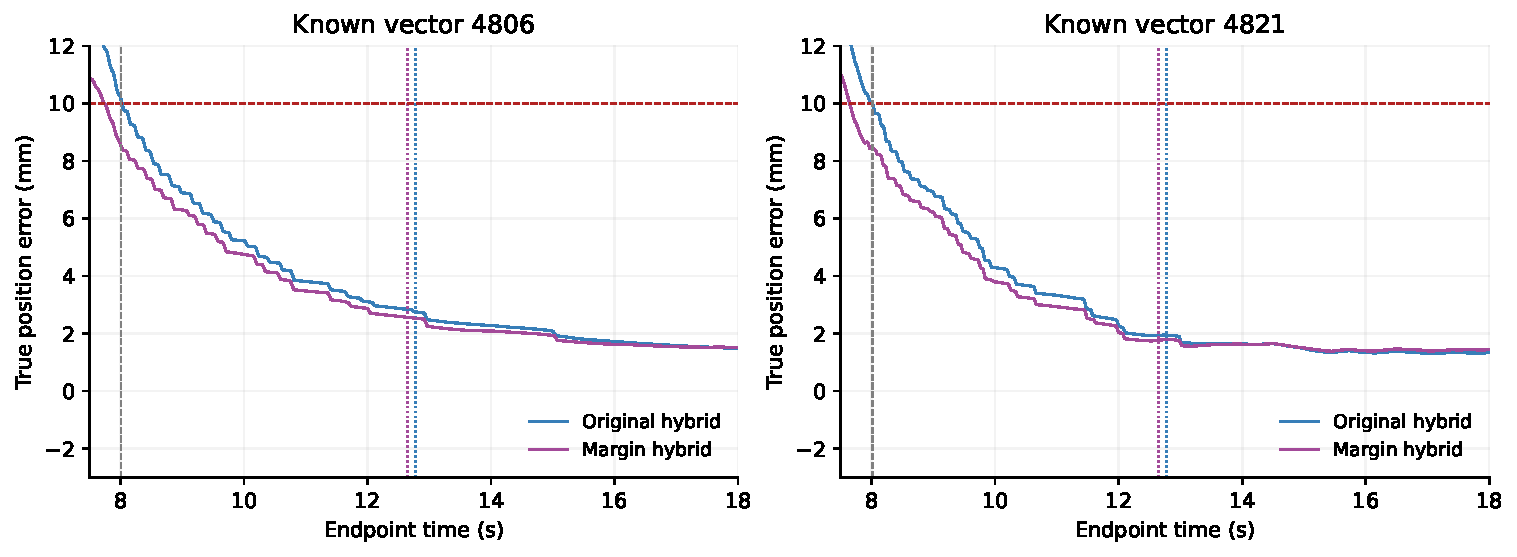
\includegraphics[width=\linewidth]{risk_extension_transition.pdf}\caption{Short diagnostic replay of the two historical failures, keeping the 1800 s temperature slope. These known-case traces locate pre-hold transition errors and are not additional successful full-horizon paths.}\label{supp:figure:1}\end{figure}

\begin{verbatim}
% Historical audit command omitted from the public source snapshot.
% Historical audit command omitted from the public source snapshot.
\end{verbatim}

\section*{S12. Supply availability and boundary-resource accounting}\renewcommand{\theHtable}{supply.\arabic{table}}

The 88-path protocol and source hashes were frozen before their outcomes. Seeds 5200--5202 are exploratory development. Those explorations use different schedules and control prototypes and do not form a paired estimate of a return-path effect. The prospective paired storage contrast uses one common supply-only flow law. The archived double-port 88-path plan was not executed and contributes no outcomes or pass count. New normal seeds are 5500--5503 and new joint seeds are 5400--5407. Gains, the availability rule and the 1/0.5 ms refinement vector are fixed. No policy is selected by this new verification.

Figure~\ref{supp:figure:2} provides the additional diagnostic graphic.
\begin{figure}[H]\centering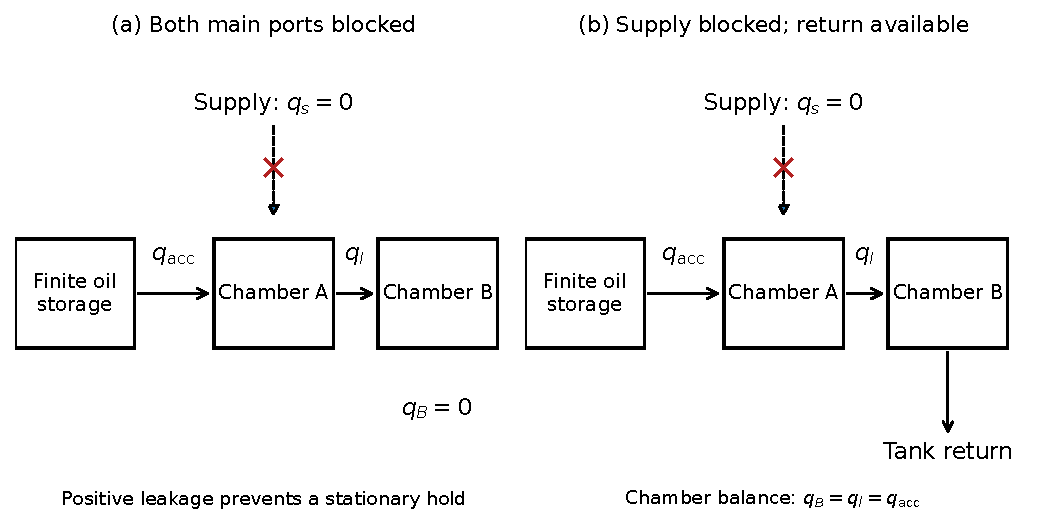
\includegraphics[width=\linewidth]{risk_extension_supply_boundary.pdf}\caption{Declared hydraulic availability boundaries. Both-port blocking prevents the steady return required by positive internal leakage. Supply disconnection leaves the shared main-valve return orifice available. These are ideal virtual interventions; valve lag and finite gas storage remain in the model.}\label{supp:figure:2}\end{figure}

\begingroup\hypersetup{hypertexnames=true}\small\setlength{\tabcolsep}{4pt}
Table~\ref{supp:longtable:3} provides the detailed supporting records.
\begin{longtable}{llrr}
\caption{All prospectively fixed joint-input intervals; SI base units unless the field name states degrees Celsius or a dimensionless scale.}\label{supp:longtable:3}\\\toprule
Class & Input & Low & High\\\midrule\endfirsthead
\toprule
Class & Input & Low & High\\\midrule\endhead
config & leakage\_scale & 3 & 8\\
config & accumulator\_flow\_scale & 0.8 & 1.2\\
config & position\_bias\_m & -0.001 & 0.001\\
config & pressure\_bias\_pa & -50000 & 50000\\
config & pressure\_noise\_scale & 1 & 1.5\\
config & temperature\_end\_c & 40 & 55\\
config & post\_step\_load\_n & 12000 & 16000\\
plant & mass\_kg & 1000 & 1400\\
plant & stiffness\_n\_m & 15000 & 21000\\
plant & viscous\_n\_s\_m & 1800 & 2600\\
plant & coulomb\_n & 680 & 1020\\
plant & stribeck\_n & 280 & 420\\
plant & effective\_bulk\_modulus\_pa & 1.6e+08 & 2.4e+08\\
\bottomrule\end{longtable}\endgroup

The following paired intervals are t-based descriptive summaries of sampled differences. The joint design stratifies 13 inputs and is not an independently drawn physical population; its intervals have no hardware-coverage or reliability interpretation. Normal-supply intervals concern four seeded noise paths at one theoretical plant. No p-values or physical pass probabilities are inferred.

\begingroup\hypersetup{hypertexnames=true}\small\setlength{\tabcolsep}{4pt}
Table~\ref{supp:longtable:4} provides the detailed supporting records.
\begin{longtable}{rrrrrrr}
\caption{Selected coordinates of all eight joint vectors. The published table lists every selected coordinate; no vector is dropped.}\label{supp:longtable:4}\\\toprule
Seed & Leak scale & x bias (mm) & p bias (kPa) & Load (kN) & Mass (kg) & $\beta_e$ ($10^8$ Pa)\\\midrule\endfirsthead
\toprule
Seed & Leak scale & x bias (mm) & p bias (kPa) & Load (kN) & Mass (kg) & $\beta_e$ ($10^8$ Pa)\\\midrule\endhead
5400 & 5.592 & -0.258 & -28.82 & 15.335 & 1264.9 & 1.685\\
5401 & 5.365 & -0.740 & 18.46 & 12.223 & 1386.5 & 2.284\\
5402 & 6.505 & 0.743 & 31.15 & 13.416 & 1239.3 & 2.029\\
5403 & 3.432 & 0.181 & -12.59 & 15.696 & 1010.2 & 1.872\\
5404 & 7.467 & 0.805 & 44.33 & 14.582 & 1104.4 & 1.744\\
5405 & 6.984 & -0.176 & 7.86 & 12.613 & 1313.4 & 2.189\\
5406 & 4.029 & -0.983 & -39.15 & 14.414 & 1084.2 & 1.988\\
5407 & 4.779 & 0.370 & -3.28 & 13.617 & 1180.7 & 2.301\\
\bottomrule\end{longtable}\endgroup

\begingroup\hypersetup{hypertexnames=true}\small\setlength{\tabcolsep}{4pt}
Table~\ref{supp:longtable:5} provides the detailed supporting records.
\begin{longtable}{rlrrrrr}
\caption{Every paired interruption outcome. Pass column is enabled/disabled (1 means pass). Error and drop are mm; oil is enabled-storage mL. Every failure remains in the calculation.}\label{supp:longtable:5}\\\toprule
Seed & Policy & Pass on/off & Error on & Error off & Drop on & Oil on\\\midrule\endfirsthead
\toprule
Seed & Policy & Pass on/off & Error on & Error off & Drop on & Oil on\\\midrule\endhead
5400 & Scalar hybrid & 1/0 & 7.811 & 17.851 & 2.551 & 205.1\\
5401 & Scalar hybrid & 1/0 & 7.752 & 21.292 & 2.734 & 280.5\\
5402 & Scalar hybrid & 1/0 & 9.215 & 32.920 & 3.154 & 375.1\\
5403 & Scalar hybrid & 1/1 & 8.142 & 8.142 & 2.594 & 0.0\\
5404 & Scalar hybrid & 1/0 & 9.070 & 45.789 & 2.939 & 549.0\\
5405 & Scalar hybrid & 1/0 & 8.116 & 39.545 & 3.356 & 464.2\\
5406 & Scalar hybrid & 1/0 & 7.453 & 9.964 & 2.534 & 131.3\\
5407 & Scalar hybrid & 1/0 & 9.089 & 25.507 & 2.968 & 288.4\\
5400 & Active PID & 1/0 & 4.966 & 19.618 & 3.515 & 241.1\\
5401 & Active PID & 1/0 & 4.865 & 23.346 & 2.232 & 282.2\\
5402 & Active PID & 1/0 & 6.241 & 32.731 & 2.608 & 387.3\\
5403 & Active PID & 1/1 & 5.244 & 7.981 & 3.997 & 94.2\\
5404 & Active PID & 1/0 & 6.169 & 45.680 & 3.088 & 547.8\\
5405 & Active PID & 1/0 & 5.052 & 39.967 & 2.832 & 481.8\\
5406 & Active PID & 1/0 & 4.450 & 12.979 & 3.108 & 162.4\\
5407 & Active PID & 1/0 & 6.127 & 28.285 & 2.919 & 336.5\\
5400 & Active SMC & 1/0 & 5.268 & 45.867 & 2.186 & 564.5\\
5401 & Active SMC & 1/0 & 5.185 & 42.406 & 1.096 & 519.2\\
5402 & Active SMC & 1/0 & 6.567 & 55.041 & 1.462 & 663.0\\
5403 & Active SMC & 1/0 & 5.560 & 31.679 & 2.471 & 377.6\\
5404 & Active SMC & 1/0 & 6.487 & 68.079 & 1.876 & 832.1\\
5405 & Active SMC & 1/0 & 5.344 & 58.241 & 1.771 & 715.1\\
5406 & Active SMC & 1/0 & 4.770 & 35.429 & 1.736 & 437.7\\
5407 & Active SMC & 1/0 & 6.448 & 45.585 & 1.638 & 549.3\\
5400 & Availability hybrid & 1/0 & 7.811 & 17.712 & 1.978 & 345.6\\
5401 & Availability hybrid & 1/0 & 7.752 & 21.169 & 1.855 & 355.9\\
5402 & Availability hybrid & 1/0 & 9.215 & 32.795 & 1.735 & 455.4\\
5403 & Availability hybrid & 1/1 & 8.142 & 8.142 & 1.867 & 245.4\\
5404 & Availability hybrid & 1/0 & 9.070 & 45.658 & 2.000 & 642.3\\
5405 & Availability hybrid & 1/0 & 8.116 & 39.453 & 2.051 & 537.7\\
5406 & Availability hybrid & 1/0 & 7.453 & 9.879 & 1.757 & 268.4\\
5407 & Availability hybrid & 1/0 & 9.089 & 25.437 & 1.971 & 427.2\\
\bottomrule\end{longtable}\endgroup

\begingroup\hypersetup{hypertexnames=true}\small\setlength{\tabcolsep}{4pt}
Table~\ref{supp:longtable:6} provides the detailed supporting records.
\begin{longtable}{@{}p{.18\linewidth}p{.25\linewidth}p{.20\linewidth}p{.12\linewidth}p{.12\linewidth}@{}}
\caption{Complete-path storage attribution. Paired changes use the same plant, noise and return path. The on/off intervention alone changes storage flow.}\label{supp:longtable:6}\\\toprule
Policy & On pass/off fail seeds & On fail/off pass seeds & Both pass & Both fail\\\midrule\endfirsthead
\toprule
Policy & On pass/off fail seeds & On fail/off pass seeds & Both pass & Both fail\\\midrule\endhead
Scalar hybrid & 5400,\allowbreak 5401,\allowbreak 5402,\allowbreak 5404,\allowbreak 5405,\allowbreak 5406,\allowbreak 5407 & None & 1 & 0\\
Active PID & 5400,\allowbreak 5401,\allowbreak 5402,\allowbreak 5404,\allowbreak 5405,\allowbreak 5406,\allowbreak 5407 & None & 1 & 0\\
Active SMC & 5400,\allowbreak 5401,\allowbreak 5402,\allowbreak 5403,\allowbreak 5404,\allowbreak 5405,\allowbreak 5406,\allowbreak 5407 & None & 0 & 0\\
Availability hybrid & 5400,\allowbreak 5401,\allowbreak 5402,\allowbreak 5404,\allowbreak 5405,\allowbreak 5406,\allowbreak 5407 & None & 1 & 0\\
\bottomrule\end{longtable}\endgroup

\begingroup\hypersetup{hypertexnames=true}\small\setlength{\tabcolsep}{4pt}
Table~\ref{supp:longtable:7} provides the detailed supporting records.
\begin{longtable}{lrrr}
\caption{Normal paired scalar-hybrid minus active-SMC differences. Units follow the metric field; negative values indicate a smaller hybrid quantity.}\label{supp:longtable:7}\\\toprule
Metric & Mean & Lower & Upper\\\midrule\endfirsthead
\toprule
Metric & Mean & Lower & Upper\\\midrule\endhead
hold\_drop\_mm & 0.3692 & -0.3315 & 1.07\\
post\_transition\_rmse\_mm & 1.019 & 1.008 & 1.031\\
post\_transition\_max\_abs\_error\_mm & 2.606 & 2.515 & 2.696\\
post\_transition\_main\_supply\_volume\_ml & -1.232e+04 & -1.246e+04 & -1.219e+04\\
accumulator\_oil\_used\_ml & 8.056 & -2.098 & 18.21\\
post\_transition\_storage\_boundary\_work\_j & 111.8 & -28.98 & 252.5\\
post\_transition\_boundary\_resource\_j & -2.586e+05 & -2.615e+05 & -2.558e+05\\
isolated\_max\_abs\_error\_mm & 0 & 0 & 0\\
\bottomrule\end{longtable}\endgroup

\begingroup\hypersetup{hypertexnames=true}\small\setlength{\tabcolsep}{4pt}
Table~\ref{supp:longtable:8} provides the detailed supporting records.
\begin{longtable}{lrrr}
\caption{Storage-enabled joint family: scalar hybrid minus active SMC. All eight pairs are included; units follow field names. Intervals are descriptive.}\label{supp:longtable:8}\\\toprule
Metric & Mean & Lower & Upper\\\midrule\endfirsthead
\toprule
Metric & Mean & Lower & Upper\\\midrule\endhead
hold\_drop\_mm & 1.074 & 0.5733 & 1.575\\
post\_transition\_rmse\_mm & 0.5502 & 0.3916 & 0.7087\\
post\_transition\_max\_abs\_error\_mm & 2.627 & 2.565 & 2.69\\
post\_transition\_main\_supply\_volume\_ml & -4364 & -4546 & -4181\\
accumulator\_oil\_used\_ml & -295.6 & -337.5 & -253.8\\
post\_transition\_storage\_boundary\_work\_j & -3454 & -4095 & -2812\\
post\_transition\_boundary\_resource\_j & -9.509e+04 & -9.935e+04 & -9.083e+04\\
isolated\_max\_abs\_error\_mm & 1.892 & 1.556 & 2.228\\
\bottomrule\end{longtable}\endgroup

\begingroup\hypersetup{hypertexnames=true}\small\setlength{\tabcolsep}{4pt}
Table~\ref{supp:longtable:9} provides the detailed supporting records.
\begin{longtable}{lrrr}
\caption{Storage-enabled joint family: availability hybrid minus scalar hybrid. All eight pairs are included; units follow field names. Intervals are descriptive.}\label{supp:longtable:9}\\\toprule
Metric & Mean & Lower & Upper\\\midrule\endfirsthead
\toprule
Metric & Mean & Lower & Upper\\\midrule\endhead
hold\_drop\_mm & -0.9521 & -1.192 & -0.7123\\
post\_transition\_rmse\_mm & -0.6262 & -0.9472 & -0.3051\\
post\_transition\_max\_abs\_error\_mm & 0 & 0 & 0\\
post\_transition\_main\_supply\_volume\_ml & -53.95 & -73.14 & -34.77\\
accumulator\_oil\_used\_ml & 123.1 & 74.97 & 171.1\\
post\_transition\_storage\_boundary\_work\_j & 1510 & 836.4 & 2184\\
post\_transition\_boundary\_resource\_j & 377.4 & -142.5 & 897.3\\
isolated\_max\_abs\_error\_mm & -2.398 & -2.986 & -1.809\\
\bottomrule\end{longtable}\endgroup

\begingroup\hypersetup{hypertexnames=true}\small\setlength{\tabcolsep}{4pt}
Table~\ref{supp:longtable:10} provides the detailed supporting records.
\begin{longtable}{llrrrrr}
\caption{Prespecified seed 5400: fine minus coarse. Steps are 0.5 and 1 ms. Pass is coarse/fine; error and drop differences are mm; supply and oil differences are mL.}\label{supp:longtable:10}\\\toprule
Policy & Store & Pass & Drop & Error & Supply & Oil\\\midrule\endfirsthead
\toprule
Policy & Store & Pass & Drop & Error & Supply & Oil\\\midrule\endhead
Scalar hybrid & on & 1/1 & -0.1996 & -0.0010 & 4.661 & -4.730\\
Scalar hybrid & off & 0/0 & -0.1554 & -0.0412 & -1.914 & 0.000\\
Active PID & on & 1/1 & -0.1892 & -0.0175 & 21.945 & -0.117\\
Active PID & off & 0/0 & -0.2120 & -0.0361 & 25.254 & 0.000\\
Active SMC & on & 1/1 & -0.0371 & -0.0042 & 4.646 & 0.976\\
Active SMC & off & 0/0 & -0.1954 & -0.1950 & -0.171 & 0.000\\
Availability hybrid & on & 1/1 & -0.1580 & -0.0010 & -2.172 & 1.444\\
Availability hybrid & off & 0/0 & -0.1496 & -0.0354 & -2.169 & 0.000\\
\bottomrule\end{longtable}\endgroup

\begingroup\hypersetup{hypertexnames=true}\small\setlength{\tabcolsep}{4pt}
Table~\ref{supp:longtable:11} provides the detailed supporting records.
\begin{longtable}{lp{.28\linewidth}p{.40\linewidth}}
\caption{All failed seeds by family and policy. Every failure is included in its summary.}\label{supp:longtable:11}\\\toprule
Family & Policy & Failed seeds\\\midrule\endfirsthead
\toprule
Family & Policy & Failed seeds\\\midrule\endhead
normal & Scalar hybrid & None\\
normal & Active PID & None\\
normal & Active SMC & None\\
normal & Availability hybrid & None\\
isolated on & Scalar hybrid & None\\
isolated on & Active PID & None\\
isolated on & Active SMC & None\\
isolated on & Availability hybrid & None\\
isolated off & Scalar hybrid & 5400, 5401, 5402, 5404, 5405, 5406, 5407\\
isolated off & Active PID & 5400, 5401, 5402, 5404, 5405, 5406, 5407\\
isolated off & Active SMC & 5400, 5401, 5402, 5403, 5404, 5405, 5406, 5407\\
isolated off & Availability hybrid & 5400, 5401, 5402, 5404, 5405, 5406, 5407\\
refined on & Scalar hybrid & None\\
refined on & Active PID & None\\
refined on & Active SMC & None\\
refined on & Availability hybrid & None\\
refined off & Scalar hybrid & 5400\\
refined off & Active PID & 5400\\
refined off & Active SMC & 5400\\
refined off & Availability hybrid & 5400\\
\bottomrule\end{longtable}\endgroup

The published article reports the normal, interruption, refinement, paired and conservation outcomes. Generated path records are intentionally omitted from the public source snapshot.

\begin{verbatim}
% Historical audit command omitted from the public source snapshot.
% Historical audit command omitted from the public source snapshot.
% Historical audit command omitted from the public source snapshot.
\end{verbatim}

\section*{S13. Equal-budget resource-oriented retuning}\renewcommand{\theHtable}{retuning.\arabic{table}}
The separate protocol fixes nine candidates and three complete 1800 s development paths per policy before any new outcome. Both policies use $g_t\in\{0.7,1.0,1.3\}$ and $g_a\in\{0.3,0.5,0.7\}$; candidate IDs follow that Cartesian-product order. Development seeds are 5600--5602. The repeated loads are $(0,9),(60,14),(300,10),(600,16),(900,11),(1200,15)$ in s/kN, with fivefold leakage, normal supply, 10 ms sensing/control and 1 ms coupled RK4. There is no retuning of the plant or observer. Failed paths rank before $B$ only in the sense that fewer failures always take priority; zero failures are required for a development-feasible candidate. Mean $B$ then ranks candidates, with ID breaking an exact tie. $B$ uses the common 8.01--1800 s window. Both policies retain the same main-valve limit and explicit 8 s latch/discharge gate. Other architecture parameters, including SMC amplitude/width and hybrid thresholds, remain fixed. This bounded search does not establish a globally optimized control-family frontier.

Selection is written to a hash-bound ledger before the independent validation tasks are executed. Validation seeds 5620--5623 are disjoint from development and all earlier normal-supply seeds. The experiment adds 54 development and eight validation paths; it does not overwrite the earlier 88-path supply study. Its normal-supply validation does not extend the interruption or joint-uncertainty evidence. The published article reports these finite protocol outcomes; the public source snapshot does not distribute the corresponding generated checkpoints.

\begingroup\hypersetup{hypertexnames=true}\small\setlength{\tabcolsep}{4pt}
Table~\ref{supp:longtable:12} provides the detailed supporting records.
\begin{longtable}{llrrrrr}
\caption{All development candidates; three paths each. Failure counts use the full feasibility screen.}\label{supp:longtable:12}\\\toprule
Policy & ID & $g_t$ & $g_a$ & Fail & Mean $B$ (kJ) & RMSE (mm)\\\midrule\endfirsthead
\toprule Policy & ID & $g_t$ & $g_a$ & Fail & Mean $B$ (kJ) & RMSE (mm)\\\midrule\endhead
Hybrid & g00 & 0.7 & 0.3 & 3 & 23.395 & 1.314 \\
Hybrid & g01 & 0.7 & 0.5 & 3 & 23.399 & 1.315 \\
Hybrid & g02 & 0.7 & 0.7 & 3 & 23.440 & 1.315 \\
Hybrid & g03 & 1.0 & 0.3 & 0 & 22.760 & 1.243 \\
Hybrid & g04 & 1.0 & 0.5 & 0 & 22.862 & 1.243 \\
Hybrid & g05 & 1.0 & 0.7 & 0 & 22.924 & 1.245 \\
Hybrid & g06 & 1.3 & 0.3 & 0 & 21.832 & 1.202 \\
Hybrid & g07 & 1.3 & 0.5 & 0 & 22.251 & 1.185 \\
Hybrid & g08 & 1.3 & 0.7 & 0 & 22.251 & 1.183 \\
SMC & g00 & 0.7 & 0.3 & 0 & 211.695 & 0.304 \\
SMC & g01 & 0.7 & 0.5 & 0 & 211.550 & 0.302 \\
SMC & g02 & 0.7 & 0.7 & 0 & 211.632 & 0.300 \\
SMC & g03 & 1.0 & 0.3 & 0 & 247.442 & 0.261 \\
SMC & g04 & 1.0 & 0.5 & 0 & 247.334 & 0.260 \\
SMC & g05 & 1.0 & 0.7 & 0 & 247.273 & 0.259 \\
SMC & g06 & 1.3 & 0.3 & 0 & 285.747 & 0.248 \\
SMC & g07 & 1.3 & 0.5 & 0 & 285.576 & 0.247 \\
SMC & g08 & 1.3 & 0.7 & 0 & 285.671 & 0.247 \\
\bottomrule\end{longtable}\endgroup
\begingroup\hypersetup{hypertexnames=true}\small\setlength{\tabcolsep}{4pt}
Table~\ref{supp:longtable:13} provides the detailed supporting records.
\begin{longtable}{llrrrrr}
\caption{Every selected-policy validation path. Error is the maximum post-transition absolute error; drop uses confirmed hold.}\label{supp:longtable:13}\\\toprule
Policy & Seed & Pass & Error (mm) & Drop (mm) & RMSE (mm) & $B$ (kJ)\\\midrule\endfirsthead
\toprule Policy & Seed & Pass & Error (mm) & Drop (mm) & RMSE (mm) & $B$ (kJ)\\\midrule\endhead
Hybrid & 5620 & 1 & 6.566 & 2.674 & 1.197 & 22.606 \\
Hybrid & 5621 & 1 & 6.917 & 2.408 & 1.204 & 22.541 \\
Hybrid & 5622 & 1 & 7.022 & 2.626 & 1.224 & 22.634 \\
Hybrid & 5623 & 1 & 6.413 & 2.215 & 1.207 & 22.079 \\
SMC & 5620 & 1 & 9.391 & 2.673 & 0.309 & 206.558 \\
SMC & 5621 & 1 & 9.809 & 2.930 & 0.308 & 211.537 \\
SMC & 5622 & 1 & 9.913 & 2.579 & 0.309 & 208.097 \\
SMC & 5623 & 1 & 9.350 & 2.835 & 0.308 & 211.070 \\
\bottomrule\end{longtable}\endgroup
Table~\ref{supp:table:13} provides the detailed supporting records.
\begin{table}[H]\centering\small
\caption{Paired hybrid minus SMC validation differences, $n=4$. Intervals use a Student $t$ multiplier with three degrees of freedom; they describe seeded simulation variability only.}\label{supp:table:13}
\begin{tabularx}{\linewidth}{@{}>{\raggedright\arraybackslash}p{.48\linewidth}XX@{}}\toprule
Metric & Mean & 95\% interval\\\midrule
Boundary resource (kJ) & -186.850 & [-190.908, -182.793] \\
Main-source volume (mL) & -8941.490 & [-9127.368, -8755.611] \\
Post-transition RMSE (mm) & 0.900 & [0.882, 0.918] \\
Confirmed-hold drop (mm) & -0.274 & [-0.825, 0.277] \\
Stored-oil discharge (mL) & 68.041 & [43.748, 92.334] \\
Mode changes & 48.000 & [48.000, 48.000] \\
\bottomrule\end{tabularx}\end{table}
The published tables summarize path metrics, including storage-outlet work, oil, mode changes, pressure and boundary counters. Candidate ranking is independent for each policy and does not equalize RMSE; lower $B$ with larger tracking error is a resource--accuracy trade-off. Four validation seeds are a small nominal screen. No finite grid certifies an optimum, physical reliability, robustness over an uncertainty region or actual energy saving.

\end{document}
